\chapter{Introducción}
\label{cap:capitulo1}
\setcounter{page}{1}

\begin{flushright}
\begin{minipage}[]{10cm}
\emph{La automatización no es el enemigo del trabajador, sino la clave para su evolución}\\
\end{minipage}\\
\end{flushright}

\vspace{1cm}

La automatización ha sido un pilar fundamental en el desarrollo de la industria moderna, permitiendo mejoras significativas en eficiencia, calidad y seguridad. Desde la Revolución Industrial hasta la actualidad, la evolución de las tecnologías ha dado paso a sistemas cada vez más sofisticados, donde la integración de robots ha transformado los entornos de producción, ofreciendo resultados de mayor calidad y reduciendo costes y tiempos de producción. En particular, la robótica industrial ha desempeñado un papel clave en sectores como la automoción, la electrónica y la manufactura, ofreciendo soluciones flexibles y altamente eficientes para la producción en serie.\\

En este capítulo se presentará el contexto en el que se desarrolla este trabajo, proporcionando una visión general de la automatización en la industria y su evolución hasta la actualidad. Posteriormente, se acotará el enfoque hacia la robótica industrial, destacando su impacto en la optimización de procesos productivos. Finalmente, se delimitará el ámbito específico de este estudio, centrado en la automatización de una línea de producción robotizada, analizando sus beneficios, retos y las tecnologías empleadas.

\section{La robótica}
\label{sec:miseccion} % etiqueta para luego referenciar esta sección

La robótica es la disciplina científica que integra conocimientos de electrónica, mecánica e informática para desarrollar sistemas automatizados capaces de realizar tareas de manera autónoma o semiautónoma. Los componentes que conforman un robot son esenciales para su funcionamiento, desde la estructura mecánica (brazos, ruedas, actuadores, etc.), que debe garantizar un movimiento preciso y estabilidad, hasta los sistemas electrónicos que deben ser totalmente compatibles y funcionales para permitir la correcta operación. Además, los algoritmos que se implementan deben ser robustos, seguros y capaces de adaptarse a diversas situaciones y condiciones del entorno. \\

En el ámbito de la robótica, los sensores juegan un papel crucial, ya que proporcionan al robot la información necesaria sobre su entorno. Estos sensores, de diversos tipos, miden una amplia gama de magnitudes físicas, como la luz, posición, desplazamiento, velocidad, aceleración, fuerza, temperatura, distancia, entre otras, funcionando de manera análoga a los órganos sensoriales en los seres humanos. \\

Una vez que los sensores recogen los datos del entorno, el software del robot procesa esta información, proporcionando la "inteligencia" necesaria para tomar decisiones. Utilizando algoritmos avanzados o inteligencia artificial, el robot es capaz de generar respuestas adecuadas a las entradas, lo que resulta en la ejecución de una acción específica, como un movimiento o la interacción con su entorno. \\

Finalmente, los actuadores son los encargados de ejecutar las acciones determinadas por el sistema de control, permitiendo que el robot lleve a cabo tareas como moverse o manipular objetos. Los actuadores son fundamentales para la efectividad del robot, ya que son los elementos que materializan las decisiones procesadas en acciones físicas tangibles. 

\begin{figure} [h!]
  \begin{center}
    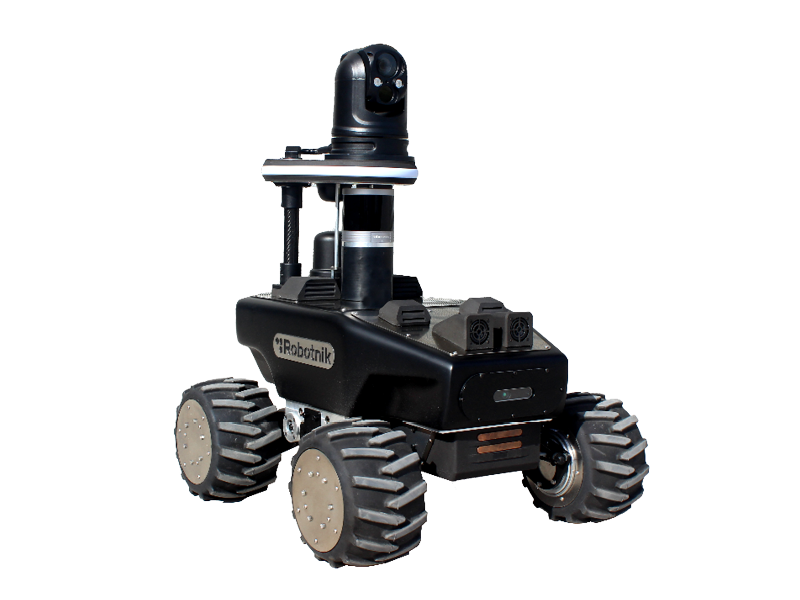
\includegraphics[width=11cm]{figs/Robot_intro}
  \end{center}
  \caption{RB-WATCHER de Robotink.}
  \label{fig:Robot_intro}
\end{figure}

\subsection{Robótica de Servicio}
\label{sec:subseccion_1}

La robótica de servicio engloba los robots diseñados para interactuar con personas o realizar tareas útiles en un entorno no industrial. Estos robots se emplean para proporcionar servicios en lugar de realizar trabajos repetitivos de manufactura, y están diseñados para facilitar tareas cotidianas, mejorar la calidad de vida o asistir a los seres humanos en áreas específicas. \\

La robótica de servicio abarca una amplia gama de aplicaciones en sectores tan diversos como la agricultura, minería, rescate, logística y conducción autónoma. Estos robots suelen ser principalmente móviles, ya que requieren desplazarse por su entorno para realizar sus tareas. Además, deben ser reactivos a las condiciones del medio y lo suficientemente robustos para garantizar el éxito de su misión, incluso en entornos impredecibles. Generalmente, estos robots tienen menos de tres grados de libertad debido a la naturaleza de las tareas que realizan, las cuales no requieren movimientos extremadamente complejos. Actúan en entornos no controlados, lo que implica que su programación y control deben ser altamente adaptativos, provocando que la programación sea especialmente compleja en ciertos escenarios.. \footnote{\url{https://udit.es/actualidad/que-es-la-robotica-de-servicio/}}. \\


\subsection{Robótica Industrial}

La robótica industrial... \\

\section{Evolución e historia de la robótica industrial}
\label{sec:segundaseccion}

\section{Conceptos fundamentales de la robótica industrial}
\label{sec:terceraseccion}

\section{Beneficios de la automatización con robots industriales}
\label{sec:cuartaseccion}

\section{Motivación del trabajo}
\label{sec:quintaseccion}

En los textos puedes poner palabras en \textit{cursiva}, para aquellas expresiones en sentido \textit{figurado}, palabras como \textit{robota}, que está fuera del diccionario castellano, o bien para resaltar palabras de una colección: \textit{(a)} es la primera letra del abecedario, \textit{(b)} es la segunda, etc.\\



No olvides incluir imágenes y referenciarlas, como la Figura \ref{fig:Robot_intro}.

\subsection{Números}
\label{sec:subseccion}

En lugar de tener secciones interminables, como la Sección \ref{sec:miseccion}, divídelas en subsecciones.

Para hablar de números, mételos en el entorno \textit{math} de \LaTeX, por ejemplo, $1.5Kg$. También puedes usar el símbolo del Euro como aquí: 1.500\euro.

\subsection{Listas}

Cuando describas una colección, usa \texttt{itemize} para ítems o \texttt{enumerate} para enumerados. Por ejemplo:

\begin{itemize}
 \item \textit{Entorno de simulación.} Hemos usado dos entornos de simulación: uno en 3D y otro en 2D.
 \item \textit{Entornos reales.} Dentro del campus, hemos realizado experimentos en Biblioteca y en el edificio de Gestión.
\end{itemize}\

\begin{enumerate}
 \item Primer elemento de la colección.
 \item Segundo elemento de la colección.
\end{enumerate}\

\paragraph{Referencias bibliográficas}
\label{sec:referencias}

Cita, sobre todo en este capítulo, referencias bibliográficas que respalden tu argumento. Para citarlas basta con poner la instrucción \verb|\cite| con el identificador de la cita. Por ejemplo: libros como \cite{vega12e}, artículos como \cite{vega19b}, URLs como \cite{vega19a}, tesis como \cite{vega18b}, congresos como \cite{vega18a}, u otros trabajos fin de grado como \cite{vega08b}.

Las referencias, con todo su contenido, están recogidas en el fichero \texttt{bibliografia.bib}. El contenido de estas referencias está en formato \texttt{BibTex}. Este formato se puede obtener en muchas ocasiones directamente, desde plataformas como \texttt{Google Scholar} u otros repositorios de recursos científicos.

Existen numerosos estilos para reflejar una referencia bibliográfica. El estilo establecido por defecto en este documento es APA, que es uno de los estilos más comunes, pero lo puedes modificar en el archivo \texttt{memoria.tex}; concretamente, cambiando el campo \verb|apalike| a otro en la instrucción \verb|\bibliographystyle{apalike}|. 

\

\

\

Y, para terminar este capítulo, resume brevemente qué vas a contar en los siguientes.
